\subsubsection*{{\titr Layout Window}}
\addcontentsline{toc}{subsubsection}{{\fehrestContent Layout Window}}

برای نشان دادن مواردی که کاربر تایپ می‌کند و محتویات فایل مورد بررسی نیاز داریم تا یک پنجره داشته باشیم تا پایه‌ریزی کلی یا layout مواردی که قرار است نشان داده شوند را در آن به نمایش بگذاریم. یک پنجره vim به طور کلی باید قادر به نمایش ۵ بخش زیر باشد که به همراه تطابق آن‌ها با تصویر آمده‌اند:

\begin{itemize}
    \item اسم فایل و وضعیت ذخیره شدن آن در دیسک (ذخیره شده/نشده)\\
    اسم فایل روبروی کلمه‌ی NORMAL آمده است. ذخیره‌نشده بودن فایل با استفاده از علامت + در کنار اسم فایل نشان داده شده است.
    \item حالت فعلی vim یا mode\\
    کلمه‌ی NORMAL در تصویر به این کار اختصاص داده شده.
    \item خط دستور یا command bar که دستوراتی که در ادامه داک می‌آیند در این قسمت وارد می‌شوند.\\
    این قسمت در آخرین خط صفحه آمده است. با زدن کلید / و یا : در حالت NORMAL کاربر شروع به تایپ در این محدوده می‌کند و تا زمانی که کلید enter را فشار نداده به این کار ادامه می‌دهد.
    \item شماره هر خط فایل\\
    این شماره‌ها در سمت چپ خطوط نوشته شده‌اند.
    \item و در نهایت محتویات فایل
\end{itemize}

ادیتور vim به صورت کلی ۳ حالت اصلی insert و normal و visual را دارد. در هر کدام از این حالت‌ها کارهای بخصوصی می‌توان انجام داد که در ادامه داک و برای هر دستور ذکر شده است که باید در کدام حالت اعمال شوند. برای گرفتن شهود بیشتر م‌یتوانید عکس زیر را مشاهده کنید که می‌تواند پیاده‌سازی مطلوبی از موارد بالا باشد.

\begin{figure}[H]
    \centerline{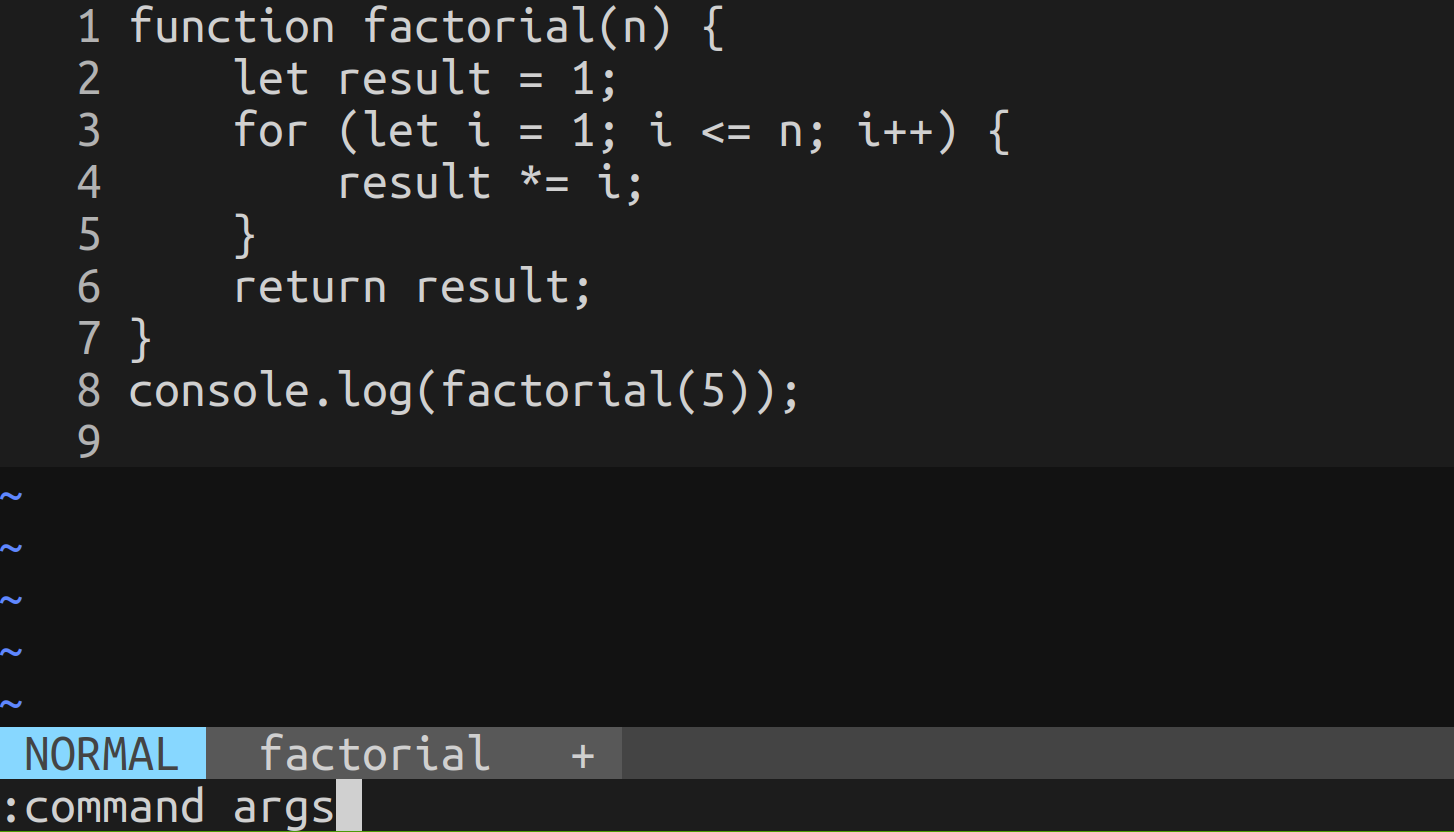
\includegraphics[width=\textwidth]{Resources/window_layout.png}}
\end{figure}

